\documentclass[11pt, a4paper]{article}

\usepackage{style}

\institution{EPFL}
\project{Semester Project}
\title{Minimal Rational Interpolation for Time-Harmonic Maxwell's Equations}
\author{Fabio Matti}
\supervisor{Prof. Fabio Nobile \\ Dr. Davide Pradovera}
\date{\today}

\begin{document}

\maketitle

\section{Abstract}
\label{sec:abstract}

\pagebreak
\section{Introduction}
\label{sec:introduction}

\pagebreak
\section{Finite element discretization of the time-harmonic Maxwell's equations}
\label{sec:maxwell}

\subsection{Vector potential formulation of the time-harmonic Maxwell's equations}
\label{subsec:maxwell-potential}

% Everything smooth enough to do all manipulations...

Let $\mathbf{E}$ denote an electric field, $\mathbf{B}$ a magnetic field
strength, $\rho$ an electric charge density, and $\mathbf{j}$ an electric
current density. Maxwell's equations are stated in \cite{monk} as
\begin{align}
    \nabla \cdot (\epsilon \mathbf{E}) &= \rho \label{equ:maxwell1} \\
    \nabla \cdot \mathbf{B} &= 0 \label{equ:maxwell2} \\
    \nabla \times \mathbf{E} &= -\partial_t \mathbf{B} \label{equ:maxwell3} \\
    \nabla \times (\mu^{-1} \mathbf{B}) &= \partial_t (\epsilon \mathbf{E}) + \mathbf{j} \label{equ:maxwell4}
\end{align}
with $\varepsilon$ being the permittivity and $\mu$ the permeability.

Equation (\ref{equ:maxwell2}) allows for an expression of the magnetic field 
$\mathbf{B} = \nabla \times \mathbf{u}$ in terms of a vector valued function
$\mathbf{u}$, the vector potential (in literature commonly denoted with
$\mathbf{A}$). Similarly, (\ref{equ:maxwell3}) suggests
rewriting the electric field $\mathbf{E} = - \nabla \phi - \partial_t \mathbf{u}$
using a scalar function $\phi$, referred to as the scalar potential.

The physical quantities $\mathbf{E}$ and $\mathbf{B}$ remain unchanged 
if we transform $\mathbf{u} \to \mathbf{u}' = \mathbf{u} + \nabla \psi$ or
$\phi \to \phi' = \phi - \partial_t \psi$ for arbitrary functions $\psi$.
A convenient choice of $\psi$ is suggested in \cite{gauge-transformation} to be
\begin{equation}
    \psi = \int_0^t \phi dt' \label{equ:gauge}
\end{equation}
which transforms $\phi \to \phi' = 0$ and $\mathbf{u} \to \mathbf{u}' = \mathbf{u}
+ \nabla \int_0^t \phi dt'$. Thus, the expressions for the electrical and
magnetic field become
\begin{align}
    \mathbf{E} &= -\partial_t \mathbf{u} \label{equ:electricfield} \\
    \mathbf{B} &= \nabla \times \mathbf{u} \label{equ:magneticfield}
\end{align}
where I renamed the variable $\mathbf{u}'$ to $\mathbf{u}$ for simplicity.

Plugging the identities (\ref{equ:electricfield}) and (\ref{equ:magneticfield})
into (\ref{equ:maxwell4}) yields 
\begin{equation}
    \nabla \times (\mu^{-1} \nabla \times \mathbf{u}) =  \varepsilon \partial_t^2 \mathbf{u} + \mathbf{j} \label{equ:maxwell-potential}
\end{equation}

For the rest of this report, I restrict myself to vector potentials $\mathbf{u}$
that exhibit a harmonic dependence on time $t$, i.e. may be factorized into
a term solely depending on the position $\mathbf{x}$ and a complex exponential:
$\mathbf{u}(\mathbf{x}, t) = \mathbf{u}(\mathbf{x}) \exp(i \omega t)$. Substituting
this expression into (\ref{equ:maxwell-potential}) results in the
\begin{equation}
    \boxed{\text{Time-harmonic potential equation:} \hspace{8pt}
     \nabla \times (\mu^{-1} \nabla \times \mathbf{u}) - \varepsilon \omega^2 \mathbf{u} = \mathbf{j}} \label{equ:maxwell-timeharmonic}
\end{equation}

\subsection{Weak formulation for the time-harmonic potential equation}
\label{subsec:maxwell-weak}

Equation (\ref{equ:maxwell-timeharmonic}) may be multiplied by a vector-valued
function $\mathbf{v} \in H_{\textrm{curl}}(\Omega)$, where
\begin{equation}
    H_{\textrm{curl}}(\Omega) = \{\mathbf{u} : \Omega \to \mathbb{C},~\text{such that}~\mathbf{u}\in L^2(\mathbb{C})^3, \nabla \times \mathbf{u} \in L^2(\mathbb{C})^3\} \label{equ:h-curl}
\end{equation}
and then integrated over all of $\Omega$ to obtain 
\begin{equation}
    \int_{\Omega} (\nabla \times ({\mu^{-1} \nabla \times \mathbf{u}})) \cdot \mathbf{v}
    - \omega^2 \int_{\Omega} \epsilon \mathbf{u} \cdot \mathbf{v} = \int_{\Omega} \mathbf{j} \cdot \mathbf{v} \label{equ:maxwell-weak-initial}
\end{equation}
% !REMINDME: Put derivation in appendix
This may further be simplified (\ref{equ:maxwell-weak-initial}) to (see Section 
\ref{sec:abstract} for details)
\begin{equation}
    \boxed{
    \int_{\Omega} ({\mu^{-1} \nabla \times \mathbf{u}}) \cdot (\nabla \times \mathbf{v})
    - \epsilon \omega^2 \int_{\Omega} \mathbf{u} \cdot \mathbf{v} 
    = \int_{\Omega} \mathbf{j} \cdot \mathbf{v}
    + \int_{\partial \Omega} (({\mu^{-1} \nabla \times \mathbf{u}}) \times \mathbf{n}) \cdot \mathbf{v}
    } \label{equ:maxwell-weak}
\end{equation}
where $\mathbf{n}$ denotes the surface normal to the boundary $\partial \Omega$.


\subsection{Two-dimensional resonant cavity}
\label{subsec:cavity}

A resonant cavity is a region $\Omega$ enclosed by a boundary $\partial \Omega$.
The boundary is subdivided into one (or more) inlets $\Gamma_N$ and a perfect
electrically conducting wall $\Gamma_D = \partial \Omega \setminus \Gamma_N$.

\begin{figure}[h]
    \centering
    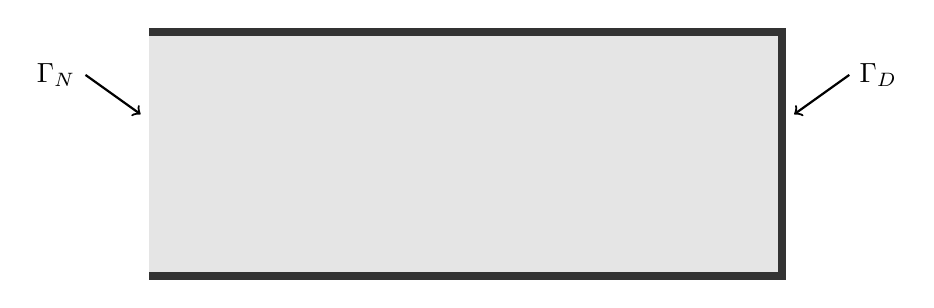
\begin{tikzpicture}
    \fill[black!80!white] (0, -0.1) rectangle (8.1, 3.1);
    \fill[black!10!white] (0, 0) rectangle (8, 3);
    \draw[thick, ->] (-0.8, 2.5) node[left] {$\Gamma_N$} to (-0.1, 2);
    \draw[thick, ->] (8.9, 2.5) node[right] {$\Gamma_D$} to (8.2, 2);
\end{tikzpicture}
    \caption{Example of a two-dimensional resonant cavity: The rectangular
    cavity.}
    \label{fig:2d-waveguide}
\end{figure}

% !REMINDME: Why only need test against v_z?!
Suppose the current density $\mathbf{j} \equiv 0$ and orient the coordinate
system in such a way that $\mathbf{u} = u_z \mathbf{e}_z$ and 
$\mathbf{v} = v_z \mathbf{e}_z$. Consequently,
\begin{equation}
    (\mu^{-1} \nabla \times \mathbf{u}) \cdot (\nabla \times \mathbf{v})
    = (\mu^{-1} \nabla u_z) \cdot (\nabla v_z)
\end{equation}
Define $g_z = (({\mu^{-1} \nabla \times \mathbf{u}}) \times \mathbf{n})_z$
along the boundary $\Gamma_N$, to convert (\ref{equ:maxwell-weak}) into
the weak formulation for a two-dimensional resonant cavity
\begin{equation}
    \int_{\Omega} (\mu^{-1} \nabla u_z) \cdot (\nabla v_z)
    - \omega^2 \int_{\Omega} \epsilon u_z v_z
    = \int_{\partial \Omega} g_z v_z \label{equ:maxwell-weak-resonant-cavity}
\end{equation}
% Boundary conditions Dirichlet and Neumann (from Monk)

\subsection{Waveguide}
\label{subsec:waveguide}

% Just j=0 and 3d, need to discuss boundary conditions

\subsection{Imperfect conductor}
\label{subsec:impedance}

% Additionally impedance boundary condition from Monk

%%% Maybe need a chapter on finite element approximation + description of usage
% of fenics or such

\pagebreak
\section{Minimal rational interpolation for the time-harmonic Maxwell's equations}
\label{sec:mri}

% General idea 

% Householder sequential algorithm

% Algorithm

% Complex root finding 

% Optimization tweaks

\pagebreak
\section{Examples}
\label{sec:examples}

\subsection{Two-dimensional rectangular cavity}
\label{subsec:examples-rectangularcavity}

% Exploratory plots

% Rational interpolation demonstration

% Analytical root finding

% Problems with non-resonant solutions suppressed by the boundary integral

% Problems with linearly combinable solutions -> Use cubby to perturb waveguide

\subsection{Dual mode circular waveguide filter}
\label{subsec:examples-dmcwf}

% Describe geometry and physical meaning

\begin{figure}[h]
    \centering
    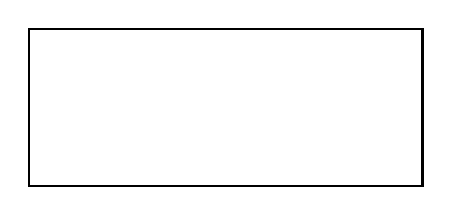
\begin{tikzpicture}
    \draw[thick] (0, 0) rectangle (5, 2);
\end{tikzpicture}
    \caption{Dual-mode circular waveguide filter.}
    \label{fig:DMCWF}
\end{figure}

% Modeling process cite rubia

% Scattering coefficient

% Measurement procedure

\subsection{Imperfectly conducting boundaries}
\label{subsec:examples-impedance}

% Pole plot

\pagebreak
\section{Conclusion and outlook}
\label{sec:conclusion}

% Danksagung

\pagebreak
\section{Appendix}
\label{sec:appendix}

\subsection{Detailed derivation for the weak formulation of the time-harmonic potential equation}
\label{subsec:derivation}

% !REMINDME: Levi-Civita tensor explanations.
The goal is to rewrite the curl-integral on the left-hand side of 
(\ref{equ:maxwell-weak-initial}):
\begin{equation}
    \int_{\Omega} (\nabla \times (\mu^{-1} \nabla \times \mathbf{u})) \cdot \mathbf{v} \label{equ:maxwell-weak-initial-LHS}
\end{equation}
In order to simplify the curls and apply the Gauss theorem, I first show prove
the vector calculus identity
\begin{equation}
    (\nabla \times \mathbf{a}) \cdot \mathbf{b} = \nabla \cdot (\mathbf{a} \times \mathbf{b}) + \mathbf{a} \cdot (\nabla \times \mathbf{b}) \label{equ:vector-calculus} \\
\end{equation}
% !REMINDME: Appropriate spaces
where $\mathbf{a}$, $\mathbf{b}$ are vector-value functions. The completely
antisymmetric tensor $\varepsilon_{ijk}$, frequently referred to as the
Levi-Civita tensor, may be employed to rewrite the components of the
curl of a vector-function $\mathbf{a}$ as the sum
% !REMINDME: Maybe lemma and proof formatting
\begin{equation}
    (\nabla \times \mathbf{a})_k = \sum_i \sum_j \varepsilon_{ijk} \partial_i u_j
\end{equation}
where $\partial_i$ denotes the partial derivative with respect to the $i$-th coordinate
direction. This yields
\begin{align}
    (\nabla \times \mathbf{a}) \cdot \mathbf{b} &= \sum_k (\nabla \times \mathbf{a})_k b_k \notag \\ 
    &= \sum_k (\sum_i \sum_j \varepsilon_{ijk} \partial_i a_j) b_k \notag \\ 
    &= \sum_k \sum_i \sum_j \partial_i (\varepsilon_{ijk} a_j b_k) - \sum_k \sum_i \sum_j a_j (\varepsilon_{ijk} \partial_i b_k) \notag \\ 
    &= \sum_k \sum_i \sum_j \partial_i (\varepsilon_{jki} a_j b_k) - \sum_k \sum_i \sum_j a_j ((-\varepsilon_{ikj}) \partial_i b_k) \notag \\ 
    &= \sum_i \partial_i (\mathbf{a} \times \mathbf{b})_i + \sum_j u_j (\nabla \times \mathbf{b})_j \notag \\ 
    &= \nabla \cdot (\mathbf{a} \times \mathbf{b}) + \mathbf{a} \cdot (\nabla \times \mathbf{b}) \label{equ:curlidentity} 
\end{align}
by expressing the scalar product as a component-sum, using the product rule and
applying the symmetry and anti-symmetry properties of the Levi-Civita tensor.
Now the identity (\ref{equ:vector-calculus}) to (\ref{equ:maxwell-weak-initial-LHS})
together with Gauss' theorem gives
\begin{align}
    \int_{\Omega} (\nabla \times ({\mu^{-1} \nabla \times \mathbf{u}})) \cdot \mathbf{v} &=
    \int_{\Omega} \nabla \cdot (({\mu^{-1} \nabla \times \mathbf{u}}) \times \mathbf{v})
    + \int_{\Omega} ({\mu^{-1} \nabla \times \mathbf{u}}) \cdot (\nabla \times \mathbf{v}) \notag \\
    &= \int_{\partial \Omega} (({\mu^{-1} \nabla \times \mathbf{u}}) \times \mathbf{v}) \cdot \mathbf{n}
    + \int_{\Omega} ({\mu^{-1} \nabla \times \mathbf{u}}) \cdot (\nabla \times \mathbf{v}) \notag \\
\end{align}

For later convenience, the boundary integral can further be simplified using
\begin{equation}
    (\mathbf{a} \times \mathbf{b}) \cdot \mathbf{c} = - (\mathbf{a} \times \mathbf{c}) \cdot \mathbf{b} \label{equ:vector-algebra}
\end{equation}
This identity follows immediately from a small manipulation with the Levi-Civita
tensor:
\begin{align}
    (\mathbf{a} \times \mathbf{b}) \cdot \mathbf{c} &= \sum_k (\sum_i \sum_j \varepsilon_{ijk} a_i b_j) c_k \notag \\
     &= \sum_j (\sum_i \sum_k (-\varepsilon_{ikj}) a_i c_k) b_j \notag \\ 
     &= - (\mathbf{a} \times \mathbf{c}) \cdot \mathbf{b} 
\end{align}
The boundary integral becomes 
\begin{equation}
    \int_{\partial \Omega} (({\mu^{-1} \nabla \times \mathbf{u}}) \times \mathbf{v}) \cdot \mathbf{n}
    = - \int_{\partial \Omega} (({\mu^{-1} \nabla \times \mathbf{u}}) \times \mathbf{n}) \cdot \mathbf{v}
\end{equation}

This concludes the short derivation, because now (\ref{equ:maxwell-weak-initial-LHS})
may be rewritten as
\begin{equation}
    - \int_{\partial \Omega} (({\mu^{-1} \nabla \times \mathbf{u}}) \times \mathbf{v}) \cdot \mathbf{n}
    + \int_{\Omega} ({\mu^{-1} \nabla \times \mathbf{u}}) \cdot (\nabla \times \mathbf{v})
\end{equation}

% 

\bibliography{biblio.bib}

\end{document}